\begin{figure}
\begin{center}
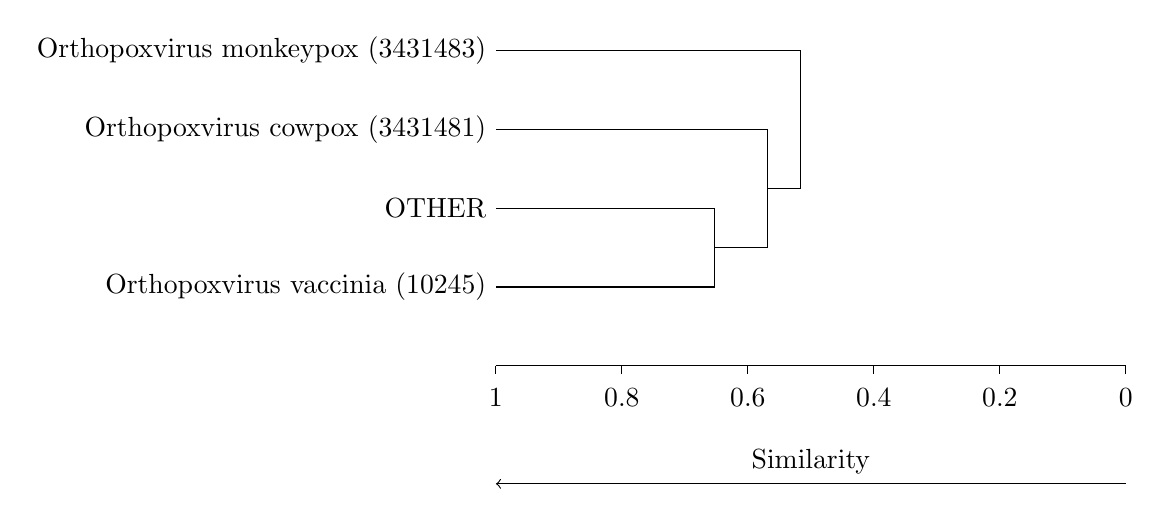
\begin{tikzpicture}[sloped,scale=1]
\draw[<-] (0,-2.500000) -- node[above]{Similarity} (8.000000,-2.500000);
\draw (0,-1.000000) -- (8.000000,-1.000000);
\draw (0.000000,-1.000000) -- (0.000000,-1.100000);
\node at (0.000000,-1.400000) {$1$};
\draw (1.600000,-1.000000) -- (1.600000,-1.100000);
\node at (1.600000,-1.400000) {$0.8$};
\draw (3.200000,-1.000000) -- (3.200000,-1.100000);
\node at (3.200000,-1.400000) {$0.6$};
\draw (4.800000,-1.000000) -- (4.800000,-1.100000);
\node at (4.800000,-1.400000) {$0.4$};
\draw (6.400000,-1.000000) -- (6.400000,-1.100000);
\node at (6.400000,-1.400000) {$0.2$};
\draw (8.000000,-1.000000) -- (8.000000,-1.100000);
\node at (8.000000,-1.400000) {$0$};
\node [anchor=east] (n3) at (0,0.000000) {Orthopoxvirus vaccinia (10245)
};
\node [anchor=east] (n4) at (0,1.000000) {OTHER};
\node (n2) at (2.775286,0.500000) {};
\node [anchor=east] (n5) at (0,2.000000) {Orthopoxvirus cowpox (3431481)
};
\node (n1) at (3.447508,1.250000) {};
\node [anchor=east] (n6) at (0,3.000000) {Orthopoxvirus monkeypox (3431483)
};
\node (n0) at (3.869699,2.125000) {};
\draw  (n0.center) |- (n1.center);
\draw  (n0.center) |- (n6.east);
\draw  (n1.center) |- (n2.center);
\draw  (n1.center) |- (n5.east);
\draw  (n2.center) |- (n3.east);
\draw  (n2.center) |- (n4.east);
\end{tikzpicture}
\caption{Orthopoxvirus (10242) [genus with 239,260 $k$-mers]\label{dendrogram10242}}
\end{center}
\end{figure}
